\documentclass[a4paper,11pt]{article}
\usepackage{amsmath,amsthm,amsfonts,amssymb,amscd,amstext,vmargin,graphics,graphicx,tabularx,multicol} 
\usepackage[francais]{babel}
\usepackage[utf8]{inputenc}  
\usepackage[T1]{fontenc} 
\usepackage{pstricks-add,tikz,tkz-tab,variations}
\usepackage[autolanguage,np]{numprint} 

\setmarginsrb{1.5cm}{0.5cm}{1cm}{0.5cm}{0cm}{0cm}{0cm}{0cm} %Gauche, haut, droite, haut
\newcounter{numexo}
\newcommand{\exo}[1]{\stepcounter{numexo}\noindent{\bf Exercice~\thenumexo} : \marginpar{\hfill /#1}}
\reversemarginpar


\newcounter{enumtabi}
\newcounter{enumtaba}
\newcommand{\q}{\stepcounter{enumtabi} \theenumtabi.  }
\newcommand{\qa}{\stepcounter{enumtaba} (\alph{enumtaba}) }
\newcommand{\initq}{\setcounter{enumtabi}{0}}
\newcommand{\initqa}{\setcounter{enumtaba}{0}}

\newcommand{\be}{\begin{enumerate}}
\newcommand{\ee}{\end{enumerate}}
\newcommand{\bi}{\begin{itemize}}
\newcommand{\ei}{\end{itemize}}
\newcommand{\bp}{\begin{pspicture*}}
\newcommand{\ep}{\end{pspicture*}}
\newcommand{\bt}{\begin{tabular}}
\newcommand{\et}{\end{tabular}}
\renewcommand{\tabularxcolumn}[1]{>{\centering}m{#1}} %(colonne m{} centrée, au lieu de p par défault) 
\newcommand{\tnl}{\tabularnewline}

\newcommand{\bmul}[1]{\begin{multicols}{#1}}
\newcommand{\emul}{\end{multicols}}

\newcommand{\trait}{\noindent \rule{\linewidth}{0.2mm}}
\newcommand{\hs}[1]{\hspace{#1}}
\newcommand{\vs}[1]{\vspace{#1}}

\newcommand{\N}{\mathbb{N}}
\newcommand{\Z}{\mathbb{Z}}
\newcommand{\R}{\mathbb{R}}
\newcommand{\C}{\mathbb{C}}
\newcommand{\Dcal}{\mathcal{D}}
\newcommand{\Ccal}{\mathcal{C}}
\newcommand{\mc}{\mathcal}

\newcommand{\vect}[1]{\overrightarrow{#1}}
\newcommand{\ds}{\displaystyle}
\newcommand{\eq}{\quad \Leftrightarrow \quad}
\newcommand{\vecti}{\vec{\imath}}
\newcommand{\vectj}{\vec{\jmath}}
\newcommand{\Oij}{(O;\vec{\imath}, \vec{\jmath})}
\newcommand{\OIJ}{(O;I,J)}


\newcommand{\reponse}[1][1]{%
\multido{}{#1}{\makebox[\linewidth]{\rule[0pt]{0pt}{20pt}\dotfill}
}}

\newcommand{\titre}[5] 
% #1: titre #2: haut gauche #3: bas gauche #4: haut droite #5: bas droite
{
\noindent #2 \hfill #4 \\
#3 \hfill #5

\vspace{-1.6cm}

\begin{center}\rule{6cm}{0.5mm}\end{center}
\vspace{0.2cm}
\begin{center}{\large{\textbf{#1}}}\end{center}
\begin{center}\rule{6cm}{0.5mm}\end{center}
}



\begin{document}
\pagestyle{empty}
\titre{Interrogation: Triangles et multiplications }{Nom :}{Prénom :}{Classe}{Date}


\exo{3} Compléter le texte suivant :\\

\bi \item 309 et 100 sont ........................................................ du ........................................................... 309 $\times$ 100.

\item Un triangle équilatéral est \reponse[2]

\item Un triangle rectangle isocèle est \reponse[2]\\
\ei

\exo{1}

\q Tracer le triangle équilatéral HGL de 6,3 cm de côté.\\
\vspace*{5,5cm}\\





\q Tracer le triangle rectangle isocèle en U tel que UV = 3,5 cm.\\
\vspace*{5,5cm}\\

\exo{2} Poser et effectuer les opérations suivantes :               

\bmul{2}

284  $\times$ 79

\vspace*{5cm}

\columnbreak

87 000 $\times$ 0,024
\vspace*{5cm}

\emul

\exo{2} Compléter par le nombre manquant :\\

\includegraphics[scale=1]{multi.eps} 


\exo{1} Entourer en bleu, pour chaque calcul, le meilleur ordre de grandeur :\\

\begin{tabular}{|c|c|c|c|c|}
\hline 
51 $\times$ 49 & 2 500 & 250 & 25 & 25 000 \\ 
\hline 
1 478 $\times$ 0,49 & 700 & 1 500 & 1 000 &  800 \\ 
\hline 
\end{tabular} 

\vspace*{1cm}



\exo{1} Une bibliothèque comporte 75 rayons et chaque rayon contient 86 livres. Calculer le nombre de livres de cette bibliothèque.\\
\reponse[5]\\

\exo{}Bonus\\
On cherche un nombre mystère. Pour cela on sait que :
\bi \item si on ajoute 2 au nombre mystère,
\item puis on multiplie le résultat par 4,
\item puis on enlève 2 au résultat,
\item alors le résultat est 34.
\ei
Quel est le nombre mystère ?








\end{document}
